\chapter{Repaso}
\section{AFD - Función de transición extendida}
Sea un AFD $D=(S,I,\delta,s^*,F)$, la función de transición extendida:
$$\widehat{\delta}:S\times I^*\rightarrow S$$
Queda definida:
\begin{itemize}
\item $\widehat{\delta}(s,\varepsilon)=s\qquad \forall s\in S$
\item $\widehat{\delta}(s,au)=\widehat{\delta}(\delta(s,a),u)\qquad a\in I,u\in I^*, s\in S$
\end{itemize}
\section{AFND - Función de transición extendida}
Sea un AFND $N=(S,I,\delta,s^*,F)$ la función de transición extendida $\widehat{\delta}$:
$$\widehat{\delta}:P(s)\times I^*\rightarrow P(s)$$
\begin{itemize}
\item $\widehat{\delta}(\phi,w)=\phi	\qquad w\in I^*$
\item $\widehat{\delta}(A,\varepsilon)=A	\qquad A\subseteq S$
\item $\widehat{\delta}(A,au)=\widehat{\delta}(\bigcup_{s\in A}\delta(s,a),u)\qquad a\in I, A\subseteq S, s\in A, u\in I^*$
\end{itemize}
\section{Equivalencia entre AFND y AFD}
Para cualquier AFND se puede construir un AFD que reconozca el mismo lenguaje, sea el AFND $N=(S,I,\delta,s^*,F)$. El AFD equivalente será $D=(S^d,I,\delta^d,s^{*d},F^d)$ en la que:

$S^d=P(S)$, donde:
\begin{itemize}
\item Para cada $X\subseteq S \land a\in I$
$$\delta^d(X,a)=\bigcup_{s\in X}\delta^d(s,a)$$
\item Para cada $a\in I, \quad \delta^d(\phi,a)=\phi$
\item $F^d=\{X\subseteq S/X\cap F\not=\phi\}$
\end{itemize}
Utilizamos el siguiente lema para probar la equivalencia.

\textbf{Lema: }Sea $D$ y $N$ los autómatas definidos anteriormente. Entonces para cada $X\subseteq S$ y $w\in I^*$
$$\widehat{\delta}^d(X,w)=\widehat{\delta}(X,w)$$

\textbf{Prueba: }Usaremos inducción sobre \textbar w\textbar. Para $w=\varepsilon$ tiene $\widehat{\delta}^d(X,\varepsilon)=\downlegend{X}{(1)}=\widehat{\delta}(X,\varepsilon)$

(1): por concepto de AFD.

Por hipótesis de inducción, para una cadena de longitud $n, w$ se cumple:
$$\widehat{\delta}^d(X,w)=\widehat{\delta}(X,w)$$

Bastará probar que $\widehat{\delta}^d(X,aw)=\widehat{\delta}(X,aw)$

\textbf{CASO I: }$X=\phi$
\begin{align*}
\widehat{\delta}^d(\phi,aw)	&=\widehat{\delta}^d(\delta^d(\phi,a),w)	\\
			&=\widehat{\delta}^d(\phi,w)\stackrel{hi}{=}\widehat{\delta}(\phi,w)	\\
			&=\phi	\\
			&\stackrel{AFND(a)}{=}\widehat{\delta}(\phi,aw)
\end{align*}

\textbf{CASO II: }$X\not=\phi$
\begin{align*}
\widehat{\delta}(X,aw) &\stackrel{b.AFD}{=}\widehat{\delta}^d(\delta^d(X,a),w)	\\
		&=\widehat{\delta}^d\left(\underbrace{\bigcup_{s\in X}\delta^d(s,a)}_{B},w\right)	\\
		&\mbox{por la construcción}	\\
		&=\widehat{\delta}^d(B,w)	\\
		&=\widehat{\delta}(B,w)	\\
		&=\widehat{\delta}\left(\bigcup_{s\in X}\delta^d(s,a),w\right)	\\
		&=\widehat{\delta}(X,aw)
\end{align*}

\textbf{Teorema: }Sea $N=(S,I,\delta,s^*,F)$ un AFND, entonces existe un AFD $D=(S^d,I,\delta^d,s^{*d},F^d)$ que es equivalente a $N$.

\textbf{Prueba: }Sea $N$ un AFND $N=(S,I,\delta,s^*,F)$ y un AFD $D=(P(S),I,\delta^d,s^{*d},F^d)$ donde $\delta^d$ y $F^d$ siguen las definiciones anteriores.

Para probar que $L(D)=L(N)$ basta probar que :
$$w\in L(D) \Leftrightarrow w\in L(N)\quad \forall w\in I^*$$

Tomemos una cadena $w\in I^*$ arbitraria, se cumple:
\begin{align*}
w\in L(D)&\Leftrightarrow \widehat{\delta}^d(s^*,w) \in F^d	\\
		&\Leftrightarrow \widehat{\delta}^d(s^*,w)\cap F^d\not=\phi	\\
		&\Leftrightarrow \widehat{\delta}(s^*,w)\cap F^d\not=\phi	\\
		&\Leftrightarrow w\in L(N)
\end{align*}

\textbf{Ejemplo: }Sea el AFND $N$ sobre $I=\{a,b\}$ dado por el D.T:
%figura 12.1
\begin{figure}[h!]
\centering
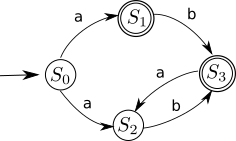
\includegraphics[width=0.4\textwidth]{img_12_1.png}
\caption{Diagrama de Transición}\label{img_12_1}
\end{figure}
Obtener el AFD $D$ equivalente.

\textbf{Solución: }Para $N: S=\{s_0,s_1,s_2,s_3\}, F=\{s_1,s_3\}, s^*=s_0$

La tabla de transición de N:
\begin{center}
\begin{tabular}{c|cc}
	&\multicolumn{2}{c}{$\delta$}	\\
	&a	&b	\\ \hline
$\phi$	&$\phi$	&$\phi$	\\
$\rightarrow s_0$ &$\{s_1,s_2\}$	&$\phi$	\\
\#$s_1$	&$\phi$	&$s_3$	\\
$s_2$	&$\phi$	&$s_3$	\\
\#$s_3$	&$s_2$	&$\phi$
\end{tabular}
\end{center}
\begin{align*}
A=\{s_1,s_2\}	\\
\delta(s_1,d)\cup\delta(s_2,d)	\\
I=\{a,b\}
\end{align*}
\begin{center}
\begin{tabular}{c|cc}
	&a	&b	\\ \hline
$\{s_0\}$	&$\{s_1,s_2\}\checkmark$	&$\phi\checkmark$	\\
$\{s_1,s_2\}$	&$\phi$	&$\{s_3\}\checkmark$	\\
$\phi$	&$\phi$	&$\phi$	\\
$\{s_3\}$	&$\{s_2\}$	&$\phi$	\\
$\{s_2\}$	&$\{\phi\}$	&$\{s_3\}$
\end{tabular}
\end{center}
%grafico 12.2
\begin{figure}[h!]
\centering
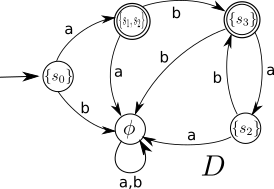
\includegraphics[width=0.5\textwidth]{img_12_2.png}
\caption{Diagrama de Transición}\label{img_12_2}
\end{figure}

\section{Conversión de un AFND -$\varepsilon$ a un AFD}
Definiremos operaciones básicas que describen computaciones en los estados de un AFND.
\begin{center}
\begin{tabular}{c|p{8cm}}
Operación	&Descripción	\\ \hline
$clausura_\varepsilon(s)$	&Conjunto de estados alcanzables desde $s$ usando solo transiciones $\varepsilon$.	\\
$clausura_\varepsilon(Q)$	&$\bigcup_{q\in Q}clausura_\varepsilon(q)$	\\
$mover(Q,a)$	&Conjuntos de estados del AFND, en los cuales hay una transición al leer el símbolo $a$ desde algún estado $q\in Q$.
\end{tabular}
\end{center}

\section{Técnica de Construcción de Subconjuntos}

\textbf{Entrada: }Un AFND $N=(S,I,\delta,s^*,F)$

\textbf{Salida: }Un AFD $D$ que acepta el mismo lenguaje $D=(S^d,I,\delta^d,s^{*d},F^d)$\\

El estado inicial de $D$ es $s^{*d}=clausura_\varepsilon(s^*)$.\\

$D_{tran}$, es la tabla de transición para $D$. $F^d$, son los estados de aceptación de $D$, son todos aquellos estados de $N$ que incluyen al menos un estado de aceptación de $N$.\\

El conjunto de estados de $D$, se denotará por $D_{estados}$.

Inicialmente, $clausura_\varepsilon(s^*)$ es el único estado de $D_{estados}$ y está sin marcar.\\
\\

\begin{algorithm}

\While {Exista un estado sin marcar Q en $D_{estados}$}{
	\For {cada símbolo de entrada} {
		$U=clausura_\varepsilon(mover(Q,a))$\\
		\If {U no esta en $D_{estados}$}{
			añadir U como un estado no marcado a $D_{estados}$		
		}
		$D_{tran}(Q,a)=U$	
	}
}
\end{algorithm}

Sea el AFND-$\varepsilon$ $N$ sobre $I=\{a,b\}$ convertido a un AFD $D$.
%grafico 12.3
\begin{figure}[h!]
\centering
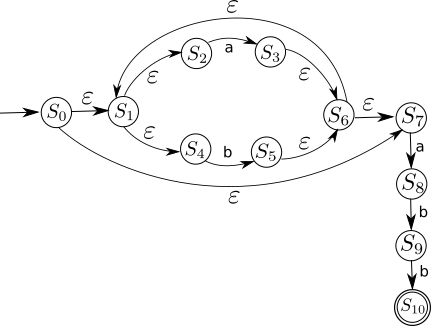
\includegraphics[width=0.65\textwidth]{img_12_3.png}
\caption{Diagrama de Transición}\label{img_12_3}
\end{figure}

Se tiene $F=\{s_{10}\}, s^*=s_0$. Hallamos $s^{*d}=clausura_\varepsilon(s_0)=\{s_0,s_1,s_2,s_4,s_7\}=A$ (sin marcar).

\begin{enumerate}
\item Marcamos $A$ y calcular:
	\begin{itemize}
	\item $D_{tran} (A,a)=clausura_\varepsilon(mover(A,a))$
	\begin{align*}
mover(A,a)=\{s_3,s_8\}	&	\\
\delta(s_0,a)=\phi \qquad &\delta(s_2,a)=s_3	\\
\delta(s_1,a)=\phi 	\qquad &\delta(s_4,a)=\phi	\\
							&\delta(s_7,a)=s_8	\\
	\end{align*}
	\begin{align*}
clausura_\varepsilon(\{s_3,s_8\})&=clausura_\varepsilon(s_3)\cup clausura_\varepsilon(s_8)	\\
				&=\{s_3,s_6,s_7,s_1,s_2,s_4\}\cup \{s_8\}	\\
				&=\{s_6,s_7,s_1,s_2,s_3,s_4,s_8\}\not = A
	\end{align*}
	Por eso lo llamaremos $B$(no marcado).

	\item $D_{tran}(A,B)=clausura_\varepsilon(mover(A,b))$
	\begin{align*}
mover(A,b)&=\{s_5\}	\\
\delta(s_4,b)	&=s_5	\\
clausura_\varepsilon(\{s_5\})&=\{s_5,s_6,s_7,s_1,s_2,s_4\}=C (no\; marcado)
	\end{align*}
	\end{itemize}
\item Marcamos $B$ y calcular.
	\begin{itemize}
	\item $D_{tran}(B,a)=clausura_\varepsilon(mover(B,a))$. Vemos el conjunto B.
	$$mover(B,a)=\{s_3,s_8\}$$
	\begin{align*}
	clausura_\varepsilon(\{s_5,s_9\})&=clausura_\varepsilon(\{s_5\})\cup clausura_\varepsilon(\{s_9\})	\\
	ignorar:	&=\{s_5,s_6,s_7,s_1,s_2,s_4,s_9\}=D (es \not= de\; B)\\
	clausura_\varepsilon(\{s_3,s_8\})	&=B(\mbox{ya lo teniamos})
	\end{align*}
	\item $D_{tran}(B,b)=clausura_\varepsilon(mover(B,b))$
	\begin{align*}
	mover(B,b)	&=\{s_5,s_9\}	\\
			&=clausura_\varepsilon(\{s_5,s_9\}=clausura_\varepsilon(\{s_5\})\cup clausura_\varepsilon(\{s_9\})	\\
			&=\{s_1,s_2,s_4,s_5,s_6,s_7,s_9\}	\\
			&=D
	\end{align*}
	\end{itemize}
\item Marcamos $C$ y calcular:
	\begin{itemize}
	\item $D_{tran}(C,a)=clausura_\varepsilon(mover(C,a))$
	\begin{align*}
	mover(C,a)	&=\{s_3,s_8\}	\\
				&=clausura_\varepsilon(\{s_3,s_8\})	\\
				&=B
	\end{align*}
	\item $D_{tran}(C,b)=clausura_\varepsilon(mover(C,b))$
	\begin{align*}
	mover(C,b)	&=\{s_5\}	\\
				&=clausura_\varepsilon(\{s_5\})=C
	\end{align*}
	\end{itemize}
\item Marcamos $D$ y calcular:
	\begin{itemize}
	\item $D_{tran}(D,a)=clausura_\varepsilon(mover(D,a))$
	\begin{align*}
	mover(D,a)	&=\{s_3,s_8\}	\\
				&=clausura_\varepsilon(\{s_3,s_8\})=B
	\end{align*}
	\item $D_{tran}(D,b)=clausura_\varepsilon(mover(D,b))$
	\begin{align*}
	mover(D,b)	&=\{s_5,s_{10}\}	\\
				&=clausura_\varepsilon(\{s_5,s_{10}\})	\\
				&=clausura_\varepsilon(\{s_5\})\cup clausura_\varepsilon(\{s_{10}\})	\\
	clausura_\varepsilon(\{s_{10}\})=\{s_{10}\}	\\
				&=clausura_\varepsilon(\{s_5,s_{10}\})	\\
				&=\{s_1,s_2,s_4,s_5,s_6,s_7,s_{10}\}=E	(s_{10}\in E)
	\end{align*}
	\end{itemize}
\item Marcamos $E$ y calcular:
	\begin{itemize}
	\item $D_{tran}(E,a)=clausura_\varepsilon(mover(E,a))$
	\begin{align*}
	mover(E,a)	&=\{s_3,s_8\}	\\
				&=clausura_\varepsilon(\{s_3,s_8\})=B	\\
	\end{align*}
	\item $D_{tran}(E,b)=clausura_\varepsilon(mover(E,b))$
	\begin{align*}
	mover(E,b)	&=\{s_5\}	\\
				&=clausura_\varepsilon(\{s_5\})=C
	\end{align*}
	\begin{center}
	\begin{tabular}{c|cc}
		&a	&b	\\ \hline
	A	&B	&C	\\
	B	&B	&D	\\
	C	&B	&C	\\
	D	&B	&E	\\
	E	&B	&C	
	\end{tabular}
	\end{center}
	%grafico 12.4
	\begin{figure}[h!]
	\centering
	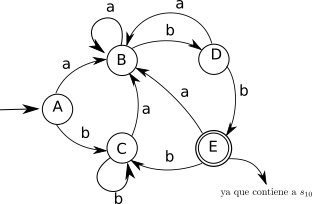
\includegraphics[width=0.5\textwidth]{img_12_4.png}
	\caption{Diagrama de Transición}\label{img_12_4}
	\end{figure}
	\end{itemize}
\end{enumerate}